\documentclass[xcolor={dvipsnames},pdf, hyperref={colorlinks=true, citecolor=ForestGreen, linkcolor=BlueViolet, urlcolor=Magenta}]{beamer}
\usetheme{Frankfurt}  
\usecolortheme{whale}
\usepackage{tikz} 
\usepackage{amsmath}
\usepackage{amsthm}
\usepackage{amssymb}              % used for \eqref{} in this document
\usepackage{dsfont}
\usepackage{hyperref}
\usepackage{threeparttable}
\usepackage{multirow}
\graphicspath{{Figures/}}
\usepackage{booktabs}
\usepackage{tikz}
\newtheorem{exmp}{Example}[section]
\usepackage{subcaption}
\usepackage{adjustbox}
\usepackage{graphicx}
\usepackage[mathscr]{euscript}
\usepackage{remreset}% tiny package containing just the \@removefromreset command
\makeatletter
\@removefromreset{subsection}{section}
\makeatother
\setcounter{subsection}{1}
\usepackage{float}
\usepackage{sgamevar}
\usepackage{sgame}

\newcommand{\defn}[1]{\textbf{#1}}


%Instructor version
\newcommand{\blank}[0]{}
\newcommand{\ddp}[1]{{\textcolor{ForestGreen}{#1}}} 
\newcommand{\dd}[1]{{\underline{\textcolor{ForestGreen}{#1}}}}

%Student version
%\newcommand{\blank}[0]{\vspace{2em}}
%\newcommand{\dd}[1]{\underline{\hspace{3cm}}} 
%\newcommand{\ddp}[1]{}

\addtobeamertemplate{navigation symbols}{}{%
	\usebeamerfont{footline}%
	\usebeamercolor[fg]{footline}%
	\hspace{1em}%
	\insertframenumber/\inserttotalframenumber
}

\section{Consumer Surplus}

%% preamble
\title{Market Equilibrium \& Efficiency}
\author{David A. D\'iaz}
\institute{UNC Chapel Hill}
\date{}

\AtBeginSection[] %Section links on slides

\begin{document} 
	
	\begin{frame}
		
		\titlepage
		
	\end{frame}
	
\begin{frame}{Welfare Economics}
	\begin{itemize}
		\item \defn{Welfare Economics}: The study of how the allocation of resources affects economic well-being.
		
		\item Today we will focus on how consumers and producers in a market are affected and will define measures of their economic well-being.
		\item In the future, we will analyze how actors outside a market can be affected.
	\end{itemize}
\end{frame}

\begin{frame}{Consumer Surplus}
	
	\begin{itemize}
		\item \defn{Willingness to pay:} The maximum amount that a buyer will pay for a good/service.
		
		\item \defn{Consumer surplus:} A measure of how well-off a buyer is due to the purchase of a good/service. Calculated as 
		
		\[CS = WTP - P\]
		
		\item Consumer surplus is used to measure the well-being of consumers. 
		
		\item In particular, it measures the benefit buyers receive from a good \textit{as the buyers themselves perceive it}.
	\end{itemize}


\end{frame}


\begin{frame}[t]{Consumer Surplus}
	

	\begin{exmp}
		\scriptsize 
		Table \ref{mookie} shows the willingness to pay of Kristina, Josh, Andrea, and Jane for one of Al's Mookie burgers (specifically, the first one they consume). If the market price of these burgers is \$5.50, what is the quantity demanded? How much consumer surplus does each consumer realize? What is the total consumer surplus in the market as a whole?
		
		\begin{table}[ht]
			\caption{WTP for Mookie Burgers}
			\label{mookie}
			\centering
			\begin{tabular}{  c|c}        
				
				Buyer   & WTP \\
				\hline
				Kristina & \$10.00 \\
				Jane & \$8.50 \\
				Josh & \$5.50 \\
				Andrea & \$4.50 \\
			\end{tabular}
		\end{table} 
	\end{exmp}
	\small
	\ddp{\pause $Q_D = 3$. Surplus/person: KV: \$4.50, Jane: \$3, Josh: \$0, Andrea: \$0. Andrea does not buy the burger since $P>WTP$. Total CS = \$7.50.\\}
	
\end{frame}


\begin{frame}[t]{Consumer Surplus}
\begin{itemize}
	\item The demand curve derived from this looks as follows:
\end{itemize}	
	\begin{figure}[H]
		\centering
		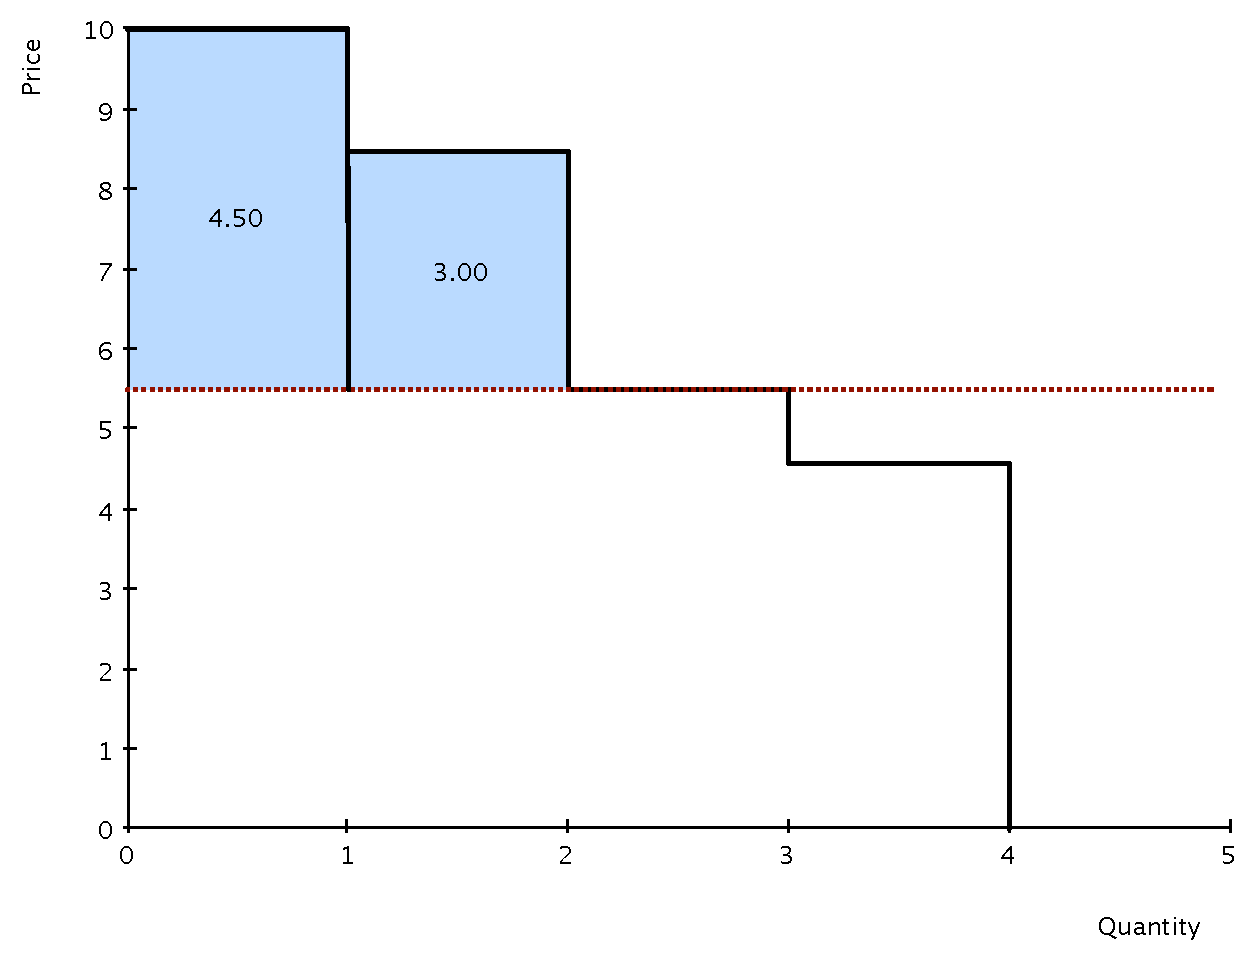
\includegraphics[scale=.25]{plot18.pdf}
		\caption{Demand for Mookie Burgers}
	\end{figure}		
	\end{frame}


\begin{frame}{Consumer Surplus}
	\begin{itemize}
		\item 	Notice that at any quantity, the demand curve shows the willingness to pay of the \textit{marginal buyer}. 
		\item Thus, we can represent consumer surplus as \dd{the area between demand and the price}.
		\item If there were enough people and the good was perfectly divisible, the steps would get smaller and smaller to eventually form a our usual demand curve.
	\end{itemize}
	\end{frame}
	
\begin{frame}{Consumer Surplus}
			\begin{exmp} 	\scriptsize Consider the demand curve for used economics textbooks for our class. If the market price was \$40, what would be the consumer surplus? What if it was \$30?
			\end{exmp}
			\begin{figure}[H]
			\centering
			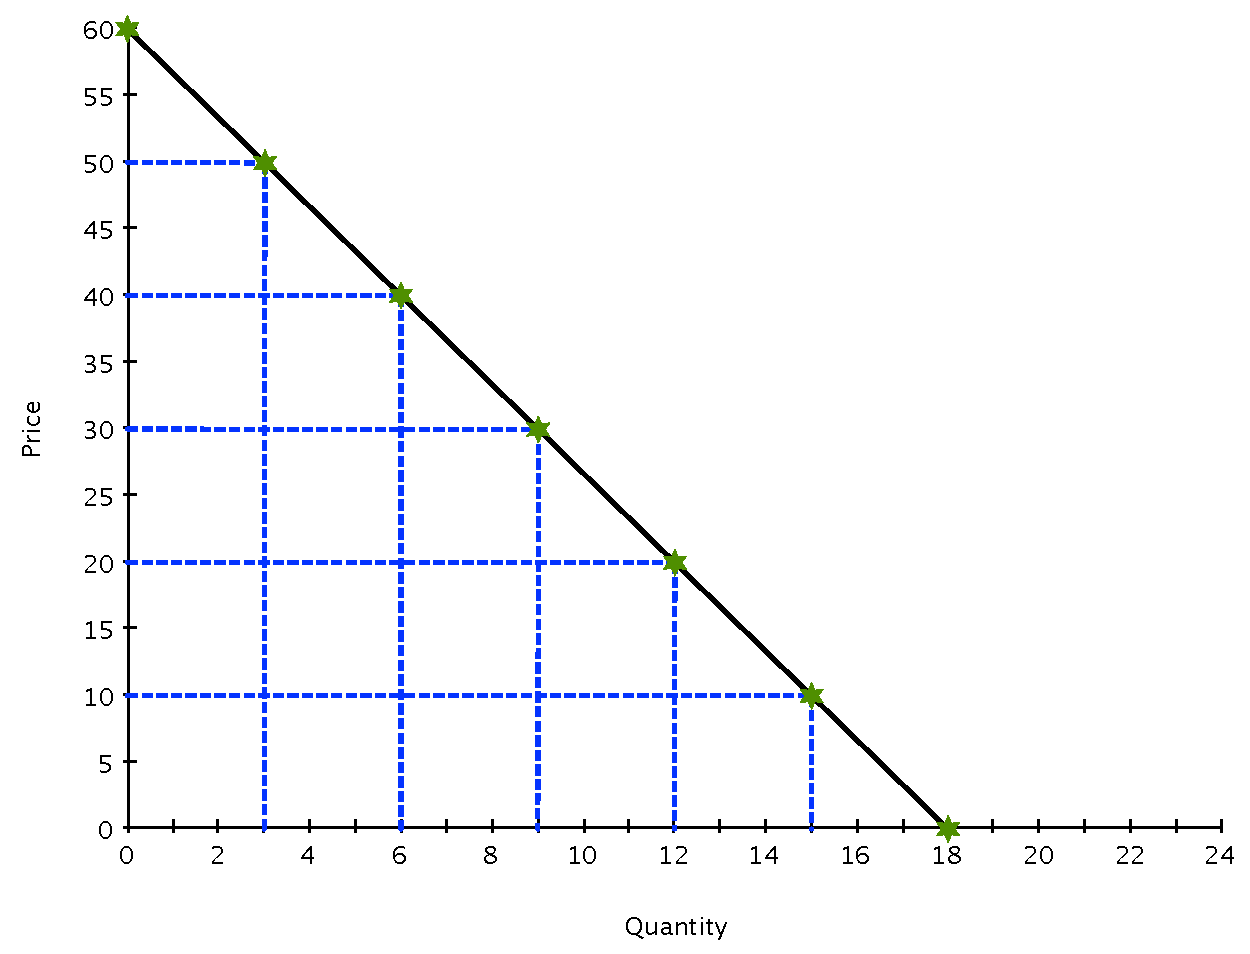
\includegraphics[scale=.25]{plot7.pdf}
			\caption{Demand for Textbooks}	
		\end{figure}
			\scriptsize	
		\pause 	\ddp{At \$40, CS = $(1/2)(20)(6) = \$60$. \\
			\pause At \$30, CS=$(1/2)(30)(9) = \$135$.}
\end{frame}
	
\begin{frame}{Consumer Surplus}
		\begin{itemize}
		\item	Notice that when prices decrease, consumer surplus \dd{increases}.  
			\begin{figure}[H]
			\centering
			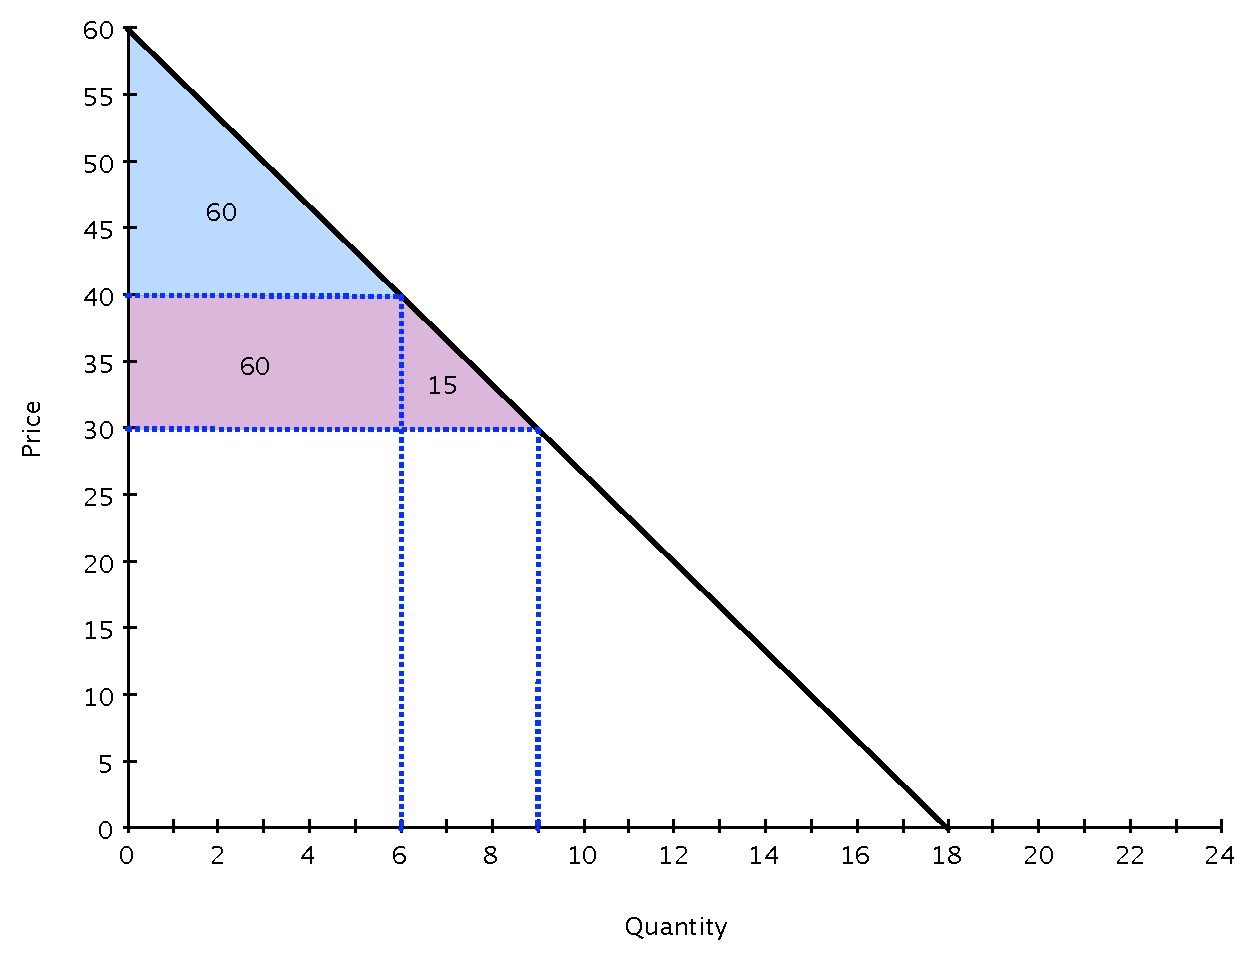
\includegraphics[scale=.25]{plot19.pdf}
			\caption{CS in the Market for Textbooks}
		\end{figure}	
			\begin{enumerate}
				\item The decrease in prices increases CS for individuals who were already purchasing the good 
				\item New buyers enter the market due to the lower price and realize CS 
			\end{enumerate}
		\end{itemize}
\end{frame}

\section{Producer Surplus}
	
		\begin{frame}{Producer Surplus}
			\begin{itemize}
			\item \defn{Seller Cost:} The value of everything a seller must give up to produce a good/service.
			\item \defn{Producer Surplus:} A measure of well-being for producers who sell a good/service. Calculated as 
			\[PS = P - SC\]
				\end{itemize}
		\end{frame}
	
\begin{frame}{Producer Surplus}
	
		\begin{exmp} 
			\small
			Consider the market for homes. There are four builders in this market, each of which can build a house with the costs shown in Table \ref{tab4}. Consider what the supply curve would look like under this cost structure. If the market price for houses is \$150,000, what is the quantity supplied and producer surplus in this market? If the price were \$250,000?
			
			\begin{table}[ht]
				\caption{Cost of Building}
				\label{tab4}
				\centering
				\begin{tabular}{ c|c}        
					
					Seller   & Cost \\
					\hline
					Ace's Builders & \$100,000 \\
					Three Brothers & \$50,000 \\
					ATP & \$200,000 \\
					Craig's Housing & \$300,000 \\
				\end{tabular}
			\end{table} 
		
		
		\end{exmp}

\end{frame}

\begin{frame}[b]{Producer Surplus }
	\begin{figure}[H]
		\centering
		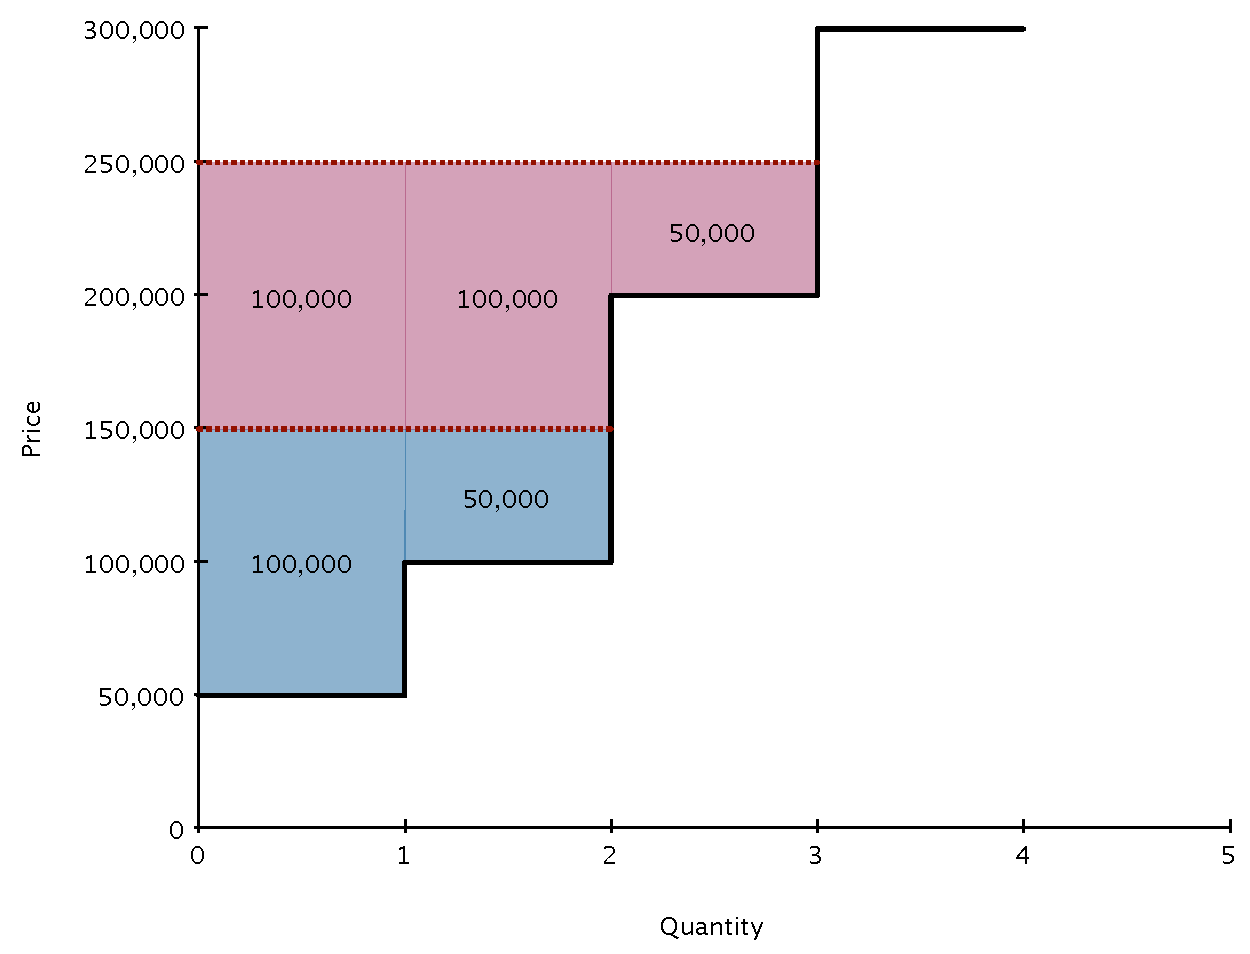
\includegraphics[scale=.25]{plot20.pdf}
		\caption{Supply of Homes}
	\end{figure}
\begin{itemize}
	\scriptsize
	\item At P = 150k: \ddp{$Q_S = 2$, PS = (150K - 50K) + (150K - 100K) = \$150K.} 
	\item At P = 250K: \ddp{$Q_S = 3$, PS = (250K - 50K) + (250K - 100K) + (250K - 200K) = \$400K.}
	\item At any quantity, the price given by the supply curve shows the cost of the \textit{marginal seller}. 
	\item Thus, we can represent producer surplus as \dd{the area b/w the price and the supply curve}.
\end{itemize}
\end{frame}


\section{Efficiency}

\begin{frame}{Efficiency}
	
\begin{itemize}
	\item 	\defn{Total Surplus:} A measure of the economic well-being of a society. \item Calculated as 
	\[TS = CS + PS = (WTP - P) + (P - SC) = WTP - SC\]
		\item Simply the value to buyers minus the cost to sellers.  
	
	\item Other actors may realize surplus from markets, even if they don't participate. We will study how that affects surplus later.
\end{itemize}
		
\end{frame}


\begin{frame}[t]{Efficiency}
	\begin{itemize}
		\item Consider a market at its equilibrium of supply and demand. Is this equilibrium allocation of resources efficient? 
		\blank\blank\blank\blank\blank
	\end{itemize}
	
	\begin{figure}[H]
		\centering
		\ddp{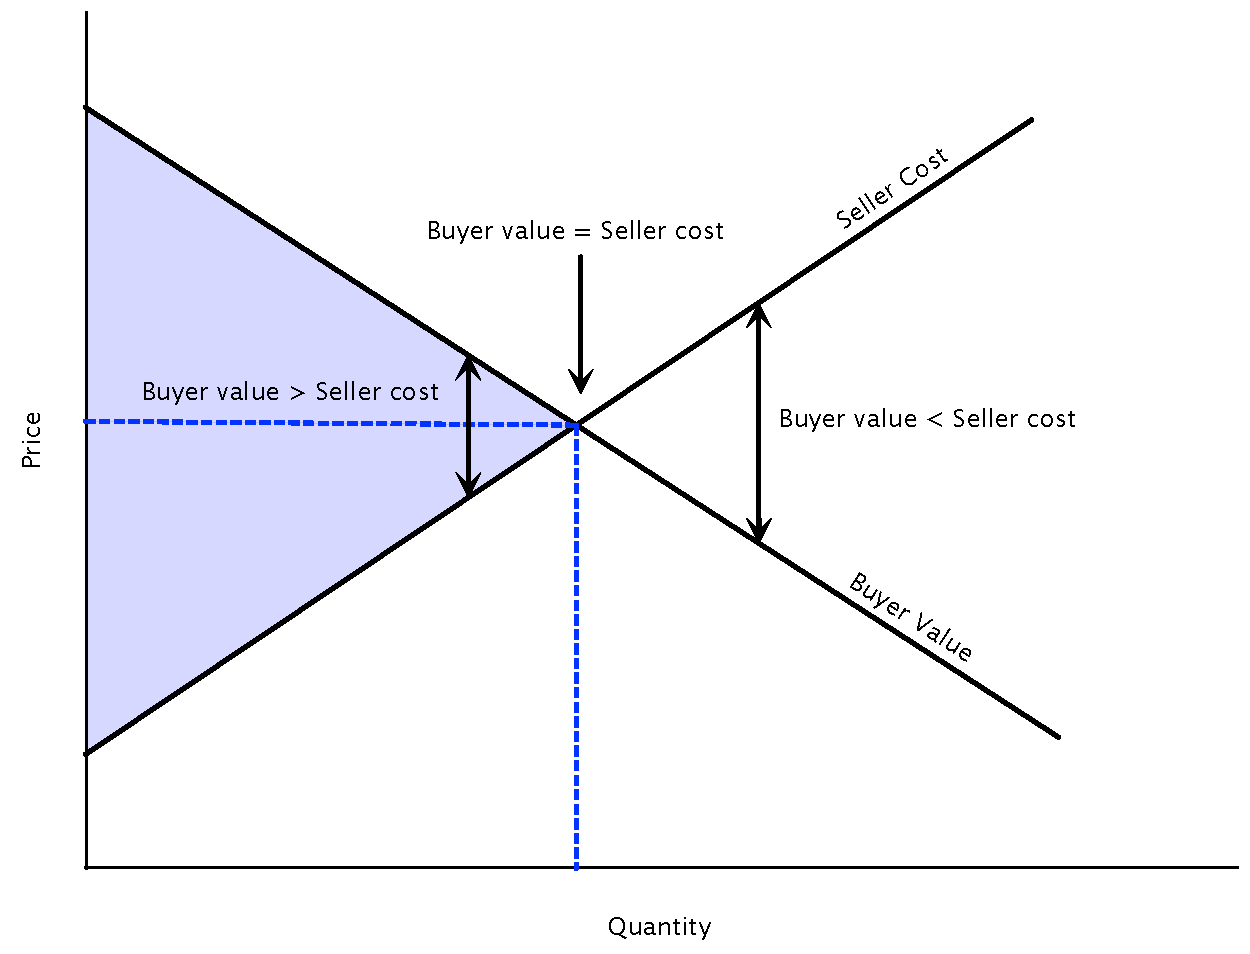
\includegraphics[scale=.25]{plot21.pdf}}
		\caption{Total Surplus at Equilibrium}
	\end{figure}
	
\end{frame}



\begin{frame}{Efficiency}
	
	\begin{itemize}
		\item Insights: 
		\begin{enumerate}
			\item Free markets allocate the supply of goods to the buyers who value them most.
			\item Free markets allocate the demand for goods to the sellers who can produce them at the lowest cost.
			\item Free markets produce the quantity of goods that maximizes the sum of consumer and producer surplus.
		\end{enumerate}
	\end{itemize}
	
\end{frame}



\begin{frame}{Efficiency}
	
	\begin{itemize}
		\item If the quantity of goods exchanged was less than the market quantity, we would have \dd{unrealized gains from trade}.
		\ddp{These are transactions for which $BV>SC$, so $TS$ would increase if these occurred.}
		\item If the quantity of goods exchanged was greater than the market quantity, we would have \dd{inefficient transactions}.
		\ddp{These are transactions for which $BV<SC$, so $TS$ would decrease if these occurred.}		
		\item \textbf{In a perfectly competitive market, the market outcome is efficient.}
	\end{itemize}
	
\end{frame}


\begin{frame}{Efficiency}
	
	\begin{exmp} 
		\scriptsize
		Table \ref{blahblah} shows the willingness to pay and seller costs of four buyers and sellers in the market for white Vans. Assume each seller has one pair of shoes to sell and each buyer only wants to buy one pair.
		\begin{table}[ht]
			\caption{Market for White Vans}
			\label{blahblah}
			\centering
			\begin{tabular}{ c|c}        
				
				WTP   & Seller Cost \\
				\hline
				\$45 & \$20 \\
				\$35 & \$40 \\
				\$60 & \$35 \\
				\$40 & \$45 \\
			\end{tabular}
		\end{table}
		
		\begin{enumerate}
			\item	What is the equilibrium price and quantity in this market? What is the value of total surplus? 
		\end{enumerate}		
	\end{exmp}
\scriptsize
 \ddp{\pause $P^* = \$40$, $Q^* = 3$
	\\ \pause $TS = WTP - SC = (60 - 20) + (45 - 35) + (40 - 40) = \$50$.}
\end{frame}

\begin{frame}{Efficiency}
	\begin{exmp}
		\scriptsize
		Table \ref{SA2} shows the willingness to pay and costs of five sellers and buyers in the market for new textbooks. Each buyer would like one textbook and each seller has one book to sell. Use the table to answer the following questions.
		
		\begin{table}[ht]
			\caption{WTP and Seller Costs for Textbooks}
			\centering
			\begin{tabular}{  c| c} 
				
				WTP   & Seller Costs \\
				\hline
				\$180 & \$85 \\
				\$150 & \$150 \\
				\$100 & \$100 \\
				\$200 & \$125 \\
				\$125 & \$60 \\
			\end{tabular}
			\label{SA2}
		\end{table}
	
		
		\begin{enumerate}
			\item What is the equilibrium price and quantity in this market?
			\item At the market equilibrium, what is the consumer, producer, and total surplus realized?			
			\item Suppose the demand curve for textbooks shifted such that each buyer values a textbook \$50 less than before. What is the new market price and quantity exchanged? What is the new total surplus?
		\end{enumerate}
	\end{exmp}
\end{frame}

\begin{frame}{Efficiency}
		\begin{table}[ht]
			\caption{WTP and Seller Costs for Textbooks}
			\centering
			\begin{tabular}{  c| c |c|c|c||c|c|c |c } 
				
				WTP   & Seller Costs & CS & PS & TS & WTP$'$ & CS$'$ & PS$'$ & TS$'$ \\
				\hline
				\$200 & \$60 & \ddp{\$75} & \ddp{\$65} & \ddp{\$140} & \ddp{\$150} & \ddp{\$50} & \ddp{\$40} & \ddp{\$90}\\
				\$180 & \$85 & \ddp{\$55} & \ddp{\$40} & \ddp{\$95} & \ddp{\$130} & \ddp{\$30} & \ddp{\$15} & \ddp{\$45}\\
				\$150 & \$100 & \ddp{\$25} & \ddp{\$25} & \ddp{\$50} & \ddp{\$100} & \ddp{\$0} & \ddp{\$0} & \ddp{\$0}\\
				\$125 & \$125 & \ddp{\$0} & \ddp{\$0} & \ddp{\$0} & \ddp{\$75} & \ddp{---} & \ddp{---} & \ddp{---}\\
				\$100 & \$150 & \ddp{---} & \ddp{---} & \ddp{---} & \ddp{\$50} & \ddp{---} & \ddp{---} & \ddp{---}\\
			\end{tabular}
			\label{SA3}
		\end{table}
	\begin{enumerate}
	\item \ddp{$(P^*,Q^*) = (\$125,4)$.}
	\item \ddp{CS = \$155, PS=\$130, TS=\$285.}
		\item \ddp{$(P^{*'},Q^{*'}) = (\$100,3)$. TS$'$=\$135.}
	\end{enumerate}
\end{frame}

\begin{frame}{Readings and Assignments}
\begin{itemize}
	\item Today: Mankiw Ch. 7
	\item Next time: Mankiw Ch. 5
	\item Problem Set 1, section 4
	\item \textbf{Homework 1 due on 5/23 by 11:55PM}
		\begin{itemize}
			\item Covers lectures 1A-2B
		\end{itemize}
\end{itemize}
\end{frame}

\end{document}